%!TEX TS-program = xelatex
% Исходная версия шаблона --- 
% https://www.writelatex.com/coursera/latex/5.1
\documentclass[c, dvipsnames]{beamer}  % [t], [c], или [b] --- вертикальное 
%\documentclass[handout, dvipsnames, c]{beamer} % Раздаточный материал (на слайдах всё сразу)
%выравнивание на слайдах (верх, центр, низ)
%\documentclass[handout, dvipsnames]{beamer} % Раздаточный материал (на слайдах всё сразу)
%\documentclass[aspectratio=169, dvipsnames]{beamer} % Соотношение сторон
\setbeamertemplate{navigation symbols}{}%remove navigation symbols

%\usetheme{Berkeley} % Тема оформленияLLL
%\usetheme{Bergen}
%\usetheme{CambridgeUS}
\usetheme{Boadilla}

\usecolortheme{crane} % Цветовая схема

%\useoutertheme{infolines} % Навигация 
%\useoutertheme{tree}
%\useoutertheme{miniframes}
%\useoutertheme{shadow}
%\useoutertheme{sidebar}
%\useoutertheme{smoothbars}
%\useoutertheme{smoothtree}
%\useoutertheme{split}
%\useoutertheme{default}


%\useinnertheme{circles}
\useinnertheme{rectangles}
%\useinnertheme{rounded}
%\useinnertheme{inmargin}


%%% Работа с русским языком
\usepackage[english,russian]{babel}   %% загружает пакет многоязыковой вёрстки
\usepackage{fontspec}      %% подготавливает загрузку шрифтов Open Type, True Type и др.
\defaultfontfeatures{Ligatures={TeX},Renderer=Basic}  %% свойства шрифтов по умолчанию
\setmainfont[Ligatures={TeX,Historic}]{Arial} %% задаёт основной шрифт документа
\setsansfont{Arial}                    %% задаёт шрифт без засечек
\setmonofont{Arial}
\usepackage{indentfirst}
\frenchspacing



%% Beamer по-русски
\newtheorem{rtheorem}{Теорема}
\newtheorem{rproof}{Доказательство}
\newtheorem{rexample}{Пример}

%%% Дополнительная работа с математикой
\usepackage{amsmath,amsfonts,amssymb,amsthm,mathtools} % AMS
\usepackage{icomma} % "Умная" запятая: $0,2$ --- число, $0, 2$ --- перечисление

%% Номера формул
\mathtoolsset{showonlyrefs=true} % Показывать номера только у тех формул, на которые есть \eqref{} в тексте.
%\usepackage{leqno} % Нумерация формул слева

%% Свои команды
\DeclareMathOperator{\sgn}{\mathop{sgn}}

%% Перенос знаков в формулах (по Львовскому)
\newcommand*{\hm}[1]{#1\nobreak\discretionary{}
{\hbox{$\mathsurround=0pt #1$}}{}}

%%% Работа с картинками
\usepackage{graphicx}  % Для вставки рисунков
\graphicspath{{images/}{images2/}}  % папки с картинками
\setlength\fboxsep{3pt} % Отступ рамки \fbox{} от рисунка
\setlength\fboxrule{1pt} % Толщина линий рамки \fbox{}
\usepackage{wrapfig} % Обтекание рисунков текстом

%%% Работа с таблицами
\usepackage{array,tabularx,tabulary,booktabs} % Дополнительная работа с таблицами
\usepackage{longtable}  % Длинные таблицы
\usepackage{multirow} % Слияние строк в таблице

%%% Программирование
\usepackage{etoolbox} % логические операторы

%%% Другие пакеты
\usepackage{lastpage} % Узнать, сколько всего страниц в документе.
%\usepackage{soul} % Модификаторы начертания
\usepackage{csquotes} % Еще инструменты для ссылок
\usepackage{multicol} % Несколько колонок


\usepackage{hyperref}
\usepackage{xcolor}
\hypersetup{        % Гиперссылки
    unicode=true,           % русские буквы в раздела PDF
    pdftitle={Заголовок},   % Заголовок
    pdfauthor={Автор},      % Автор
    pdfsubject={Тема},      % Тема
    pdfcreator={Создатель}, % Создатель
    pdfproducer={Производитель}, % Производитель
    pdfkeywords={keyword1} {key2} {key3}, % Ключевые слова
    colorlinks=true,        % false: ссылки в рамках; true: цветные ссылки
    linkcolor=,          % внутренние ссылки
    citecolor=green,        % на библиографию
    filecolor=magenta,      % на файлы
    urlcolor=blue           % на URL
} 

\usepackage{dcolumn}

%fffff3
\definecolor{backgr}{RGB}{146,26,29}
\definecolor{backgr1}{RGB}{230,43,37}
\definecolor{ex1}{RGB}{231,142,36}
\definecolor{ex2}{RGB}{249,155,28}
\definecolor{ex3}{RGB}{242,103,36}

\definecolor{red}{RGB}{230,43,37}
%\setbeamercolor{normal text}{fg=black,bg=backgr}
\setbeamercolor{frametitle}{bg=backgr,fg=white}
%\setbeamercolor{footline}{bg=backgr,fg=white}
%\setbeamercolor{normal text}{bg=yellow}
%\setbeamercolor{section in toc}{fg=yellow}
%\setbeamercolor{subsection in toc}{fg=blue}

% How to change colour of Navigation Bar in Beamer -  много интересного

%Пример команд, задающих внешний вид блока
\setbeamercolor{block title}{fg=white,bg=ex1}
\setbeamerfont{block title}{family=\sffamily}
\setbeamercolor{block body}{bg=white}
\setbeamertemplate{blocks}[rounded][shadow=fasle]
\setbeamercolor{title}{bg=backgr, fg=white}
\setbeamercolor{alerted text}{fg=backgr1}

\newlength\subtitwd
\setlength\subtitwd{4cm}% change the width here

\makeatletter
\newcommand\titlegraphicii[1]{\def\inserttitlegraphicii{#1}}
\titlegraphicii{}
\newcommand\superviser[1]{\def\insertsuperviser{  #1}}
\superviser{}

\setbeamertemplate{title page}
{
  \vbox{}
   {\usebeamercolor[fg]{titlegraphic} \hspace{0.35ex} \inserttitlegraphic\hfill\inserttitlegraphicii \hspace{1ex} \par }\vspace{1.5ex}
  \begin{centering}
    \begin{beamercolorbox}[sep=8pt,center]{institute}
      \usebeamerfont{institute}\insertinstitute
    \end{beamercolorbox}
    \begin{beamercolorbox}[sep=8pt,center]{title}
    
      \usebeamerfont{title}\inserttitle\par%
      \ifx  \insertsubtitle\@empty%
      \else%
        \vskip0.5em%
        {\usebeamerfont{subtitle}\usebeamercolor[fg]{subtitle}\insertsubtitle\par}%
      \fi%     
    \end{beamercolorbox}%
    \vskip1em\par
    \begin{beamercolorbox}[sep=5pt,center]{date}
      \usebeamerfont{date}\insertdate
    \end{beamercolorbox}%\vskip0.5em
    \begin{beamercolorbox}[sep=5pt,center]{author}
      \usebeamerfont{author}\insertauthor
    \end{beamercolorbox}
        \begin{beamercolorbox}[sep=4pt,center]{institute}
      \usebeamerfont{institute}\insertsuperviser
    \end{beamercolorbox}
  \end{centering}
  %\vfill
}
\makeatother

\setbeamercolor{item projected}{bg=ex3}
\setbeamertemplate{enumerate items}[default]

\setbeamercolor{palette primary}{bg=white}
\setbeamercolor{palette primary}{fg=black}
\setbeamercolor{palette secondary}{bg=white}
\setbeamercolor{palette secondary}{fg=black}
\setbeamercolor{palette tertiary}{bg=white}
\setbeamercolor{palette tertiary}{fg=black}

\setbeamercolor{itemize item}{fg=ex3}
\setbeamercolor{itemize subitem}{fg=ex2}
\setbeamercolor{itemize subsubitem}{fg=ex1}

\setbeamercolor{enumerate item}{fg=ex3}
\setbeamercolor{enumerate subitem}{bg=ex3}
\setbeamercolor{enumerate subsubitem}{bg=ex3}


\setbeamertemplate{itemize subitem}{$\Rightarrow$}
\setbeamertemplate{itemize item}{$\blacktriangleright$}



\usepackage{todo}
\newcolumntype{a}{>{\columncolor{red}}c}


\usefonttheme{professionalfonts}

\title[R\&D Investment, Exporting, and \\	Productivity Dynamics]{R\&D Investment, Exporting, and \\	Productivity Dynamics}
%\subtitle{Защита выпускной квалификационной работы}


 \usepackage{amsmath}

\author[Касьянова Ксения]{Касьянова Ксения \\ \smallskip \scriptsize ЭО-15-01 }


%\author[Имя автора]{Имя автора \\ \smallskip \scriptsize \href{mailto:author@ranepa.ru}{author@ranepa.ru} \\ \smallskip  \href{http://ranepa.ru}{http://ranepa.ru} }

\institute[РАНХиГС]{ \uppercase{
  Российская Академия Народного Хозяйства и  \\ Государственной Службы при Президенте Российской Федерации}}
\date{}


\titlegraphic{
\includegraphics[scale=0.5]{logo1}}
\titlegraphicii{
\includegraphics[scale=0.5]{logo2}}

\begin{document}

\frame[plain]{\titlepage}	% Титульный слайд




\section{Motivation:}

\begin{frame}[shrink=3]
\frametitle{\insertsection} 
\begin{block}{Research question:}
	\begin{itemize}
		%		\item  Улучшить прогноз ВВП России с помощью иерархических моделей. 
		\item   Does openness to trade promote productivity?
	\end{itemize}
	
\end{block}


\begin{block}{Motivation:}



Exports and firm productivity are correlated
\begin{itemize}
	\item   Selection: robust finding
	\item  Learning-by-Exporting: mixed evidence
	
\end{itemize} 


Interdependent R\&D and exporting at firm-level
\begin{itemize}
	\item   Exporting → larger market → more R\&D incentive
	\item  Selection
	\item R\&D → higher expected future productivity → re-inforce
	selection
	
\end{itemize}

Market size effect depend on
\begin{itemize}
	\item   domestic/exporting profitability
	\item  innovation process
	\item  costs assoicated with each activity
	
\end{itemize}

\end{block}



\end{frame}


%\begin{frame}[shrink=3]
%\frametitle{\insertsection} 
%
%
%
%
%• Document firm-level R\&D and export dynamics in Taiwanese
%Electronics Industry.
%
%• Estimate an empirical structural model and quantify how optimal R\&D and export decisions depend on expectation of future productivity/export demand; fixed/sunk costs assoicated with choices
%
%• Decompose correlated R\&D and Export dynamics by
% selection on unobservables;
% state dependence
%
%• To be done: quantify how large is the market size effect, i.e. how
%does R\&D respond to trade cost reduction?
%
%\end{frame}
%
%
%


\section{Literature}


\begin{frame}[shrink=3]
\frametitle{\insertsection} 

\begin{enumerate}
	\item Empirics on exporting and productivity: Bernard and Jensen (1999); Bustos (2007)
\item  Recent macro/trade models of joint decisions of R\&D and export:
Atkeson and Burstein (2008); Constantini and Melitz (2008)
\item  Structural estimation of industry equilibrium:
Olley and Pakes (1996): productivity dynamics;
Das, Roberts and Tybout (2007): exporting with sunk and
fixed costs

\item  A reflection of a new mechanism: endogenous innovation?
 Bustos (2007), Lileeva and Trefler (2007): trade liberalization induces more innovation;
 Aw, Roberts, and Winston (2007): R\&D and exporting
correlated.

\end{enumerate}


\end{frame}




\section{Theoretical Model}





\begin{frame}[shrink=3]
\frametitle{\insertsection} 

\textbf{Technology:}

• Short-run marginal cost:

$$lnc_{it} = lnc(k_{it},w_{t}) − x_{it} = \beta_0 + \beta_{k }lnk_{it} +\beta_{w} lnw_{t} − x_{it}$$

• $k_{it }$ capital stock, $w_{t}$ variable input price, $x_{it}$ productivity
• Differs across firms, but not a function of output
• Two sources of heterogeneity: capital-observable, productivity-not
observable by researchers.

\end{frame}


\begin{frame}[shrink=3]
\frametitle{\insertsection} 


\textbf{Demand:}

• Demand for the firm’s output in domestic market (Dixit -Stiglitz)
$$q^D_{it} = Q^D_t(p^D_{it} /P^D_t)^{\eta_D} = \dfrac{I^D_t}{P^D_t} \left( \dfrac{p^D_{it}}{P^D_t} \right)^{\eta_D} = \Phi^D_t (p^D_{it} )^{\eta_D}$$ 

• All aggregates are combined into $\Phi^D_t$

• Similarly, demand for the firm’s output in export market:

$$q^X_{it} = Q^X_t(p^X_{it} /P^X_t)^{\eta_X} = z_{it} \dfrac{I^X_t}{P^X_t} \left( \dfrac{p^X_{it}}{P^X_t} \right)^{\eta_X} = \Phi^X_t z_{it} (p^X_{it} )^{\eta_X}$$ 


• $z_{it}$: firm-specific demand shock in export market. Heterogeneity
between export and domestic market for each firm.

\end{frame}

\begin{frame}[shrink=3]
\frametitle{\insertsection} 

• These assumptions imply domestic and export revenue function as:

$$ln r^D_{it} = (\eta_D + 1) ln( \frac{\eta_D}{\eta_D + 1}) + ln \Phi^D_t + (\eta_D + 1)lnc_{it}$$

$$ln r^X_{it} = (\eta_X + 1) ln( \frac{\eta_X}{\eta_X + 1}) + ln \Phi^X_t + (\eta_X + 1)lnc_{it} + z_{it}$$

• Profits: directly relate revenue to unobservables $x_{it}$ and $z_{it}$.

$$\pi^D_{it} = (−1/\eta_D)r^D_{it} (\Phi^D_t, k_{it}, x_{it})$$

$$\pi^X_{it} = (−1/\eta_X)r^X_{it} (\Phi^X_t, k_{it}, x_{it}, z_{it})$$



Finally, total cost $tvc_{it} = r^D_{it} (1 + \frac{1}{\eta_D}) + r^X_{it} (1 + \frac{1}{\eta_X})$

\end{frame}




\begin{frame}[shrink=3]
\frametitle{\insertsection} 

• Productivity $x_{it}$ evolves endogenously, depending on R\&D $d_{it−1}$
and exporting $e_{it−1}$:
$$x_{it} = g(x_{it−1}, d_{it−1}, e_{it−1}) + \psi_{it}$$

• $d_{it−1}$: learning-by-investing. $e_{it−1}$: learning-by-exporting. $d, e$: discrete (0/1) or continuous.

• Export demand shock $z_{it}$ evolves exogenously as a first order markov process:
$$z_{it} = \rho_z z_{it−1} + \mu_{it}, \mu_{it} \sim N(0, \sigma^2_{\mu}$$

• Firm size measure capital $k_i$: short time series dimension with very little variation over time


\end{frame}





\begin{frame}[shrink=3]
\frametitle{\insertsection} 

\textbf{Sources of dynamics:}

• $e$ and $d$ affect evolution of future $x$; $z$ is persistent over time

• Beginning each activity involves one-time sunk cost.

Sequence of Information and Decisions:

\begin{enumerate}
	\item  Begin period t with productivity and export demand shock $(x_{it}, z_{it})$.
\item  Random fixed cost $\gamma^F_{it}$ of exporting and sunk cost $γ^S_{it} \to$  export decision.
\item  Maximize static profits $\pi^D_{it}$ and, if exporting, $\pi^X_{it}$.
\item  Random fixed cost of R\&D $\gamma^I_{it}$ and sunk cost $\gamma^D_{it} \to$ R\&D decision.
\item  End of period t, new states $(x_{it+1}, z_{it+1})$ realized.

\end{enumerate}
\end{frame}





\begin{frame}[shrink=3]
\frametitle{\insertsection} 


\begin{figure}
	\centering
	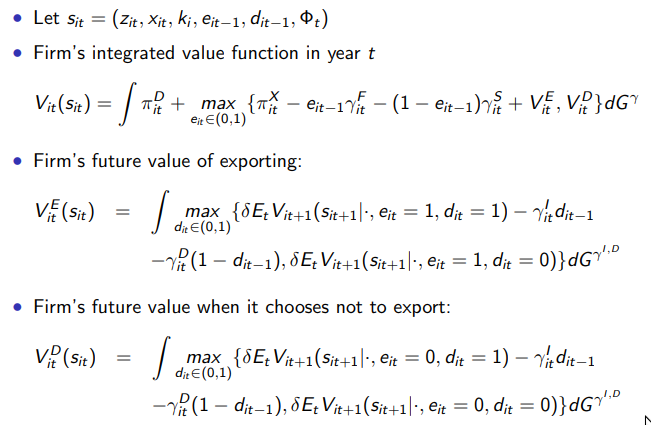
\includegraphics[width=0.7\linewidth]{screenshot004}


	\label{fig:screenshot004}
\end{figure}



\end{frame}




\begin{frame}[shrink=3]
\frametitle{\insertsection} 


Firm’s problem:


$$ \max_{\{e_{t},d_{t}\}} \left\{ E_0 \sum^\infty_{t=0} \delta^t \left\{ \pi^D(\omega_t) +e_t [\pi^X(\omega_t,z_t)-\gamma^X(e_{t-1})] -d_t\gamma^R(d_{t-1})\right\}\right\}$$

subject to productivity evolution:

$$\omega_t = g(\omega_{t−1}, e_{t−1}, d_{t−1})$$


\begin{itemize}
	\item No static optimization
\item 
High $\omega_t$ affects incentives for both $e_t$ and $d_t$
\item 
Interactions between $e_t$ and $d_t$ through both objective
function and productivity dynamics
\item 
Persistence through sunk versus fixed costs (both iid): option
value of waiting


\end{itemize}
\end{frame}



\begin{frame}[shrink=3]
\frametitle{\insertsection} 


\begin{figure}
	\centering
	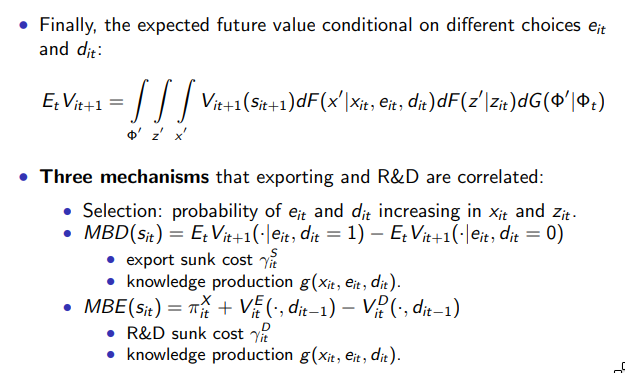
\includegraphics[width=0.7\linewidth]{screenshot005}
	
	
	\label{fig:screenshot005}
\end{figure}



\end{frame}








\section{Estimation}




\begin{frame}[shrink=3]
\frametitle{\insertsection} 


Static equations:

\begin{itemize}
	\item $\{tvc_{it},r^D_{it},r^X_{it}\}$ to estimate elasticity of demand
\item 
$\{r^D_{it}, k_{it}, m_{it}, n_{it}\}$ to estimate productivity $\omega_{it}$
\item 
$ \{r^X_{it}, \omega_{it}\}$ to estimate export demand shock $z_{it}$
\end{itemize}

Productivity dynamics:
$$\omega_{it} = g(\omega_{it−1}, e_{it−1}, d_{it−1})$$
Estimated by OLS using a parametric assumption about $g(·)$

Dynamic exporting and investment decisions:

$\{e_{it}, d_{it}|z_{it}\}$ to estimate parameters of the model (sunk and fixed costs) using ML

\end{frame}




\begin{frame}[shrink=3]
\frametitle{\insertsection} 

\begin{figure}
	\centering
	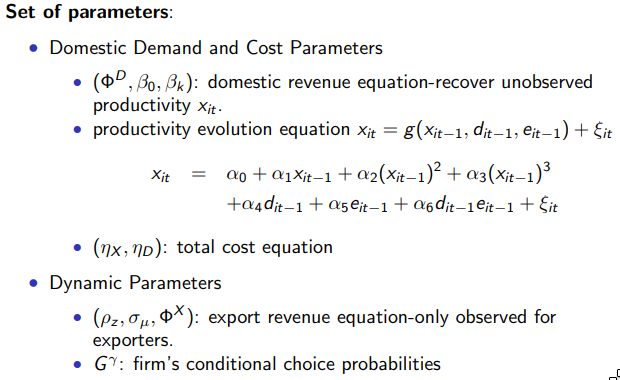
\includegraphics[width=0.7\linewidth]{screenshot006}
	\label{fig:screenshot006}
\end{figure}

\end{frame}




\begin{frame}[shrink=3]
\frametitle{\insertsection} 

\begin{figure}
	\centering
	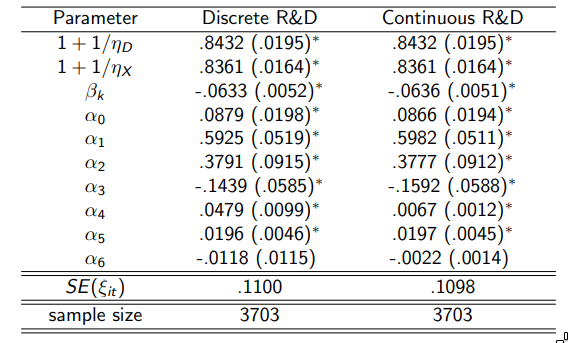
\includegraphics[width=0.7\linewidth]{screenshot007}
	\label{fig:screenshot007}
\end{figure}

\begin{figure}
	\centering
	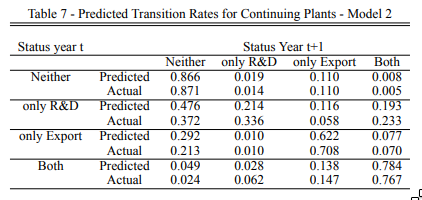
\includegraphics[width=0.7\linewidth]{screenshot009}
	\label{fig:screenshot009}
\end{figure}


\end{frame}


\section{Data}

\begin{frame}[shrink=3]
\frametitle{\insertsection} 

Taiwanese Electronics Industry

• Balanced panel of 1,237 plants for 2000-2004


• Product classes: consumer electronics, telecommunication
equipment, computers and storage equipment, electronics parts and
components.

• Most dynamic industry in Taiwanese manufacturing sector
\begin{itemize}
	\item   Export participation .39 - compete with low-margins
	\item  R\&D performers .17 - major focus on process innovation
	\item  Significant cross-sectional heterogeneity in productivity and
	activities.
	\item  Sustained productivity growth, 3.6\% annual in 80s and 90s.
	
\end{itemize}

Key variables: Revenue-domestic and export, Physical capital stocks
(size), R\&D expenditure, Variable costs-material, labor, energy


\end{frame}


\begin{frame}[shrink=3]
\frametitle{\insertsection} 


• Transition pattern of R\&D and exporting:

\begin{figure}
\centering
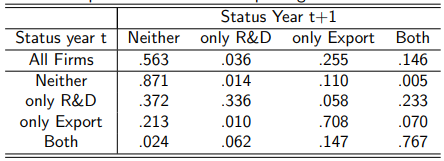
\includegraphics[width=0.7\linewidth]{screenshot002}
\label{fig:screenshot001}
\end{figure}


• Persistence in the status: (1) high sunk costs (2) high degree of
persistence in the underlying profit heterogeneity.

• Exporting is more common than R\&D investment.

• Undertaking one of the activities in year t→ more likely to add the
other in year t + 1, less likely to drop the other in year t + 1


\end{frame}


\section{Estimation}


\begin{frame}[shrink=3]
\frametitle{\insertsection} 

\begin{figure}
	\centering
	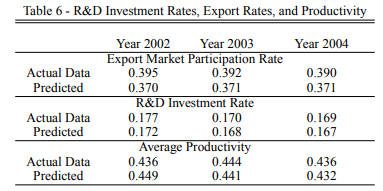
\includegraphics[width=0.7\linewidth]{screenshot008}
	\label{fig:screenshot008}
\end{figure}


\end{frame}






\section{Results}




\begin{frame}[shrink=3]
\frametitle{\insertsection} 


Productivity dynamics (estimation of $g(·)$):
$$\dfrac{ \delta \omega_{it}>0}{\delta e_{it-1}} > 0; \dfrac{\delta\omega_{it}}{\delta_{it−1}}> 0; \dfrac{\delta^2\omega_{it}}{\delta e_{it}\delta d_{it}}< 0$$

Sunk and Fixed costs of Exporting and R\&D:
\begin{itemize}
	\item  R\&D costs roughly twice as big as Export costs
\item  Sunk costs are roughly twice as big as Fixed costs
\item  Around 10\% of revenues

\end{itemize}

Interdependence between exporting and investment:
\begin{itemize}
	\item  Selection based on $\omega_{it}$ for both $e_{it}$ and $d_{it}$
\item  A lot of persistence due to large sunk costs relative to fixed
costs
\item  Probability of exporting decreasing in R\&D and probability of
investment decreases in export status due to the interaction in
the productivity dynamics

\end{itemize}


\end{frame}


\begin{frame}[shrink=3]
\frametitle{\insertsection} 

• Productivity in response to both R\&D and exporting.

• Impact of R\&D is larger.

• But, relatively low exporting cost makes it a more important
channel.

• The interdependence of R\&D and exporting is dominated by
selection: stable export demand.



\end{frame}


\end{document}